\chapter{화학 평형}
        \section{평형 상수}
        \hspace{\parindent} 자발적인 반응이 일어날 때 Gibbs 에너지는 감소하는 방향으로 이동한다. 일정한 압력과 온도에서 Gibbs 
        에너지가 최소가 될 때까지 반응이 일어나는 경향성이 존재한다. $A\rightleftharpoons B$ 반응을 생각하자. A가 B로 매우 작은 
        양 $\difform \xi$만큼 변화할 때, A의 변화량 $\difform n_A = -\difform \xi$이고, B의 변화량 
        $\difform n_B = \difform \xi$이다. 이때 $\xi$는 \textbf{반응 진척도(Extent of reaction)}이다. 반응 
        진척도는 몰수로 나타낸다. \textbf{반응 Gibbs 에너지(Reaction Gibbs energy, $\Delta_r G$)}는 다음과 같이 정의된다:
        \begin{defn}[반응 Gibbs 에너지]\label{rxngibbs}
        \begin{equation*}
            \Delta_r G=\left(\frac{\partial G}{\partial \xi}\right)_{p,T}
        \end{equation*}
        \end{defn}
        따라서 $\difform \xi$만큼 반응이 진행되었을 때, 반응의 Gibbs 에너지는 다음과 같이 변화한다:
        \begin{equation*}
            \difform G =\mu_A \difform n_A + \mu_B \difform n_B = \left(\mu_B-\mu_A\right)\difform \xi
        \end{equation*}
        따라서 다음과 같은 식이 성립한다:
        \begin{equation*}
            \begin{aligned}
                \left(\frac{\partial G}{\partial \xi}\right)_{p,T} &= \mu_B-\mu_A \\
                \Delta_r G &= \mu_B - \mu_A
            \end{aligned}
        \end{equation*}
        이때 $\mu_A > \mu_B$일 때 $A\rightarrow B$ 반응이 자발적이고, $\mu_A < \mu_B$일 때 $B \rightarrow A$ 반응이 자발적이다. 
        만약 $\mu_A = \mu_B$, 즉 $\Delta_r G =0$일 때에는, 반응이 평형에 도달한다. 따라서 다음과 같은 사실이 성립한다:
        \begin{enum}
            \item $\Delta_r G<0$일 때, 정반응이 자발적이다.
            \item $\Delta_r G>0$일 때, 역반응이 자발적이다.
            \item $\Delta_r G=0$일 때, 반응은 평형 상태이다.
        \end{enum}
        $\Delta_r G<0$인 반응을 \textbf{에너지 방출(Exergonic)} 반응이라고 한다. 이는 자발적 반응이 일어나면 다른 반응을 일으킬 수 있음을 
        함의한다. 반대로 $\Delta_r G>0$인 반응을 \textbf{에너지 흡수(Endergonic)} 반응이라고 한다. 이는 반응을 일으키기 위해서는 에너지를 
        공급해야 함을 함의한다.
        \par 이상 기체에서 $A \rightleftharpoons B$ 반응이 일어날 때, $\Delta_r G$는 다음과 같다:
        \begin{equation*}
            \begin{aligned}
                \Delta_r G &=\mu_B -\mu_A = \left(\mu_B^\circlehbar + RT\ln{\frac{p_B}{p^\circlehbar}}\right) - \left(\mu_A^\circlehbar + RT\ln{\frac{p_A}{p^\circlehbar}}\right)\\
                &= \Delta_r G^\circlehbar + RT\ln{\frac{p_B}{p_A}}
            \end{aligned}
        \end{equation*}
        이때 \textbf{반응 지수(Reaction quotient, $Q$)}는 $Q=\frac{p_B}{p_A}$로 쓸 수 있다. 반응 지수는 분자가 0일 때 $Q=0$부터 
        분모가 0일 때 $Q=\infty$까지 존재한다. 표준 상태에서 표준 반응 Gibbs 에너지는 다음과 같이 정의한다:
        \begin{equation*}
            \Delta_r G^\circlehbar = G_m^\circlehbar\left(B\right)-G_m^\circlehbar\left(A\right)=\mu_B^\circlehbar-\mu_A^\circlehbar
        \end{equation*}
        실제 적용에서는 다음과 같이 계산한다:
        \begin{equation*}
            \Delta_r G^\circlehbar = \Delta_f G^\circlehbar \left(B\right)-\Delta_f G^\circlehbar \left(A\right)
        \end{equation*}
        만약 평형 상태, 즉 $\Delta_r G = 0$일 때 반응 지수 $Q$는 평형 상수 $K$와 같아진다. 따라서
        \begin{equation*}
            RT \ln{K}=-\Delta_r G^\circlehbar, K=\left(\frac{p_B}{p_A}\right)_\mathrm{equilibrium}
        \end{equation*}
        가 성립한다. 이때 혼합 Gibbs 에너지를 고려하지 않으면 $\xi$에 대해 $\Delta_r G^\circlehbar$은 선형적인 관계를 보이나, 혼합을 
        고려하면 아래로 볼록한 곡선이 된다. 따라서 혼합까지 고려한 최솟값이 반응의 평형점이 된다.
        \par 화학종 J에 대해, 반응식은 다음과 같이 나타낼 수 있다:
        \begin{equation*}
            0=\sum_\mathrm{J} \nu_\mathrm{J} \mathrm{J}
        \end{equation*}
        이때 $\nu$는 반응물일 때 (-), 생성물일 때 (+)이다. 일반적인 반응의 Gibbs 에너지는 다음과 같이 구할 수 있다: $\difform \xi$만큼 
        반응이 진행되었을 때, $\difform G = \sum_J \mu_J \difform n_J$에서
        \begin{equation*}
            \difform G = \sum_J \mu_J \nu_J \difform \xi = \left(\sum_J \mu_J \nu_J\right)\difform \xi
        \end{equation*}
        가 성립한다. 그리고 $\Delta_r G=\left(\frac{\partial G}{\partial \xi}\right)_{p,T}$에서,
        \begin{equation*}
            \Delta_r G = \sum_\mathrm{J} \nu_\mathrm{J} \mu_\mathrm{J}
        \end{equation*}
        가 성립한다. 이제 $\mu_J = \mu_J^\circlehbar +RT\ln{a_J}$를 도입하자.
        \begin{equation*}
            \begin{aligned}
                \Delta_r G &= \sum_J \nu_J \mu_J^\circlehbar + RT\sum_J \nu_J \ln{a_J}\\
                &= \Delta_r G^\circlehbar +RT\sum_J \nu_J \ln{a_J}\\
                &= \Delta_r G^\circlehbar +RT\sum_J \ln{{a_J}^{\nu_J}}
            \end{aligned}
        \end{equation*}
        이때 $\sum_i \ln{x_i} = \ln{\prod_i x_i}$가 성립하므로, 다음이 성립한다:
        \begin{equation*}
            \Delta_r G = \Delta_r G^\circlehbar + RT\ln{\prod_J {a_J}^{\nu_J}}
        \end{equation*}
        이때 반응 지수를 다음과 같이 정의한다:
        \begin{defn}[반응 지수]
        \begin{equation*}
            Q = \prod_J {a_J}^{\nu_J}
        \end{equation*}
        \end{defn}
        따라서 $Q = \left(\text{생성물의 활동도 곱}\right)/\left(\text{반응물의 활동도 곱}\right)$의 꼴을 가지게 된다. 
        따라서 일반적인 반응 Gibbs 에너지는 다음과 같다:
        \begin{obs}[반응 Gibbs 에너지와 반응 지수의 관계]
        \begin{equation*}
            \Delta_r G = \Delta_r G^\circlehbar + RT \ln{Q}
        \end{equation*}
        \end{obs}
        \par 이때 표준 반응 Gibbs 에너지는 다음과 같다:
        \begin{obs}[표준 반응 Gibbs 에너지]
        \begin{equation*}
            \Delta_r G^\circlehbar = \sum_J \nu_J \Delta_f G^\circlehbar \left(J\right)
        \end{equation*}
        \end{obs}
        평형 상태에서는 $\Delta_r G =0$이고 $Q=K$이므로, 다음이 성립한다:
        \begin{defn}[열역학적 평형 상수]
        \begin{equation*}
            K=\left(\prod_J {a_J}^{\nu_J}\right)_\mathrm{equilibrium}
        \end{equation*}
        \end{defn}
        이렇게 표현된 평형 상수를 \textbf{열역학적 평형 상수(Thermodynamic equilibrium constant)}라 한다. 활동도는 다음 표와 같이 쓸 수 있다:
        \begin{table}[H]
        \centering
            \begin{tabular}{ c c c c }
                \hline
                \rowcolor{lightgray}
                상태 & 측정값 & 활동도에 대한 근사 & 정의 \\
                \hline
                용질 & 몰랄 농도 & $b_J / b_J^\circlehbar$ & $b^\circlehbar = 1 \text{ mol kg}^{-1}$\\
                & 몰 농도 & $\left[J\right]/c^\circlehbar$ & $c^\circlehbar=1\text{ mol dm}^{-3}$\\
                기체 & 부분 압력 & $p_J/p^\circlehbar$ & $p^\circlehbar= 1\text{ bar}$ \\
                순수한 고체나 액체 & & $1$ (정의) & \\
                \hline
            \end{tabular}
        \end{table}
        따라서 평형 상수와 반응 Gibbs 에너지 사이에 다음이 성립한다:
        \begin{law}[평형 상수와 반응 Gibbs 에너지 사이의 관계]
        \begin{equation*}
            \Delta_r G^\circlehbar = -RT\ln{K}
        \end{equation*}
        \end{law}
        \par 위 표에서 살펴본 것과 같이, 평형 상수는 여러 종류의 변수로 나타낼 수 있다. 이는 활동도 계수를 각 변수마다 다르게 정의함으로써 해결할 수 있다. 예를 들어 
        몰 분율을 이용할 경우 $a_J = \gamma_J x_J$, 몰랄 농도를 이용할 경우 $a_J = \gamma_J b_J/b^\circlehbar$, 몰 농도를 이용할 경우 
        $a_J = \gamma_J \left[ J \right]/c^\circlehbar$로 정의할 수 있다. 이때 $A+B\rightleftharpoons C+D$ 반응이 있다고 하면, 몰랄 농도를 이용할 때 평형 상수는 다음과 같다:
        \begin{equation*}
            K = \frac{a_C a_D}{a_A a_B} = \frac{\gamma_C \gamma_D}{\gamma_A \gamma_B}\times\frac{b_C b_D}{b_A b_B} = K_\gamma K_b
        \end{equation*}
        이때 활동도 계수는 평형 상태에서 결정해야 한다. 많은 경우에 $K_\gamma = 1$로 가정하여 $K \approx K_b$로 두고 풀 수 있다.
        \par 만약 기체 반응일 경우, 평형 상수 결정에 압력을 이용할 수 있다. 이때 평형 상수는 다음과 같이 계산된다:
        \begin{obs}[압력 평형 상수]
        \begin{equation*}
            \begin{aligned}
                K &= \prod_J {a_J}^{\nu_J} = \prod_J \left(\frac{p_J}{p^\circlehbar}\right)^{\nu_J} = \prod_J \left[J\right]^{\nu_J}\left(\frac{RT}{p^\circlehbar}\right)^{\nu_J}\\
                &= \prod_J \left[J\right]^{\nu_J}\times\prod_J \left(\frac{RT}{p^\circlehbar}\right)^{\nu_J}
            \end{aligned}
        \end{equation*}
        \end{obs}
        따라서 무차원 평형 상수 $K_c$는 다음과 같이 정의된다:
        \begin{equation*}
            K_c = \prod_J\left(\frac{\left[J\right]}{c^\circlehbar}\right)^{\nu_J}
        \end{equation*}
        따라서
        \begin{equation*}
            K= K_c \times \prod_J\left(\frac{c^\circlehbar RT}{p^\circlehbar}\right)^{\nu_J}
        \end{equation*}
        가 성립한다. 이때 $\Delta \nu = \sum_J \nu_J$라 하면, 다음이 성립한다:
        \begin{equation*}
            K = K_c \times \left(\frac{c^\circlehbar RT}{p^\circlehbar}\right)^{\Delta\nu}
        \end{equation*}
        계산을 위해서는, $p^\circlehbar / c^\circlehbar R = 12.03$ K로 두면 된다.
        \par Boltzmann 분포로 평형을 해석할 경우, $A\rightarrow B$ 반응이 흡열 반응이라 할 때 A의 에너지 준위와 B의 에너지 준위의 분포가 비슷하면(즉 $\Delta_r S \approx 0$) 
        A가 더 우세할 것이다. 그러나 B의 에너지 준위가 A의 에너지 준위보다 더 촘촘하면(즉 $\Delta_r S > 0$) B가 더 우세할 것이다. 구체적으로, 
        $\Delta_r G^\circlehbar = \Delta_r H^\circlehbar - T \Delta_r S^\circlehbar$이므로 다음이 성립한다:
        \begin{equation*}
            K = e^{-\frac{\Delta_r H^\circlehbar}{RT}}\times e^{\frac{\Delta_r S^\circlehbar}{R}}
        \end{equation*}
        따라서 흡열 반응일 경우 $K$를 낮추는 효과가 있고, 한편 반응 엔트로피가 양수일 경우 $K$를 높이는 효과가 있다.
    \section{평형 이동}
        \hspace{\parindent} Henry Louis Le Chatelier는 다음과 같은 이론을 세웠다\textbf{(Le Chatelier의 원리(Le Chatelier's principle))}:
        \begin{law}[Le Chatelier의 원리]
        평형에 있는 계에 변화가 생기면 그 변화의 영향을 최소화하는 방향으로 반응한다.
        \end{law}
        \par 평형 상수는 $\Delta_r G^\circlehbar$에 의존한다. 이때 $\Delta_r G^\circlehbar$는 특정 압력에서 정의되고, 즉 평형 상수는 온도에만 의존한다. 
        평형 상태에 있는 계에 비활성 기체를 추가하거나 용기의 부피를 바꾸면서 기체의 부분 압력을 바꾸면, 평형 상수를 맞추기 위해 평형이 이동한다. $A\rightleftharpoons 2B$ 
        평형이 용기 안에서 일어나고 있다고 하자. 이때 평형 상수는 다음과 같다:
        \begin{equation*}
            K = \left(\frac{{p_B}^2}{p_A p^\circlehbar}\right)_\mathrm{equilibrium}
        \end{equation*}
        만약 기체의 부분 압력이 증가할 경우, 증가한 압력을 낮추기 위해 $A \leftarrow 2B$ 반응이 지배적으로 일어난다. 반대로 기체의 부분 압력이 감소하면, 
        감소한 압력을 올리기 위해 $A \rightarrow 2B$ 반응이 지배적으로 일어난다.
        \par 분해도(Degree of dissociation) $\alpha$에 대해, 처음에 A 분자만 $n$만큼 존재한다면, 평형 상태에서는 A 분자가 $\left(1-\alpha\right)n$만큼 존재하고 
        B 분자가 $2\alpha n$만큼 존재하게 된다. 이때 평형 상태에서 각각의 몰 분율은
        \begin{equation*}
            x_A = \frac{n_A}{n_\mathrm{tot}}=\frac{\left(1-\alpha\right)n}{\left(1-\alpha\right)n+2\alpha n}=\frac{1-\alpha}{1+\alpha}, x_B = \frac{2\alpha}{1+\alpha}
        \end{equation*}
        이때 평형 상수는 
        \begin{equation*}
            K=\frac{{p_B}^2}{p_A p^\circlehbar}=\frac{{x_B}^2 p^2}{x_A p p^\circlehbar}=\frac{4\alpha^2 \left(p/p^\circlehbar\right)}{1-\alpha^2}
        \end{equation*}
        이고, $p$는 총 압력이다. 따라서 다음이 성립한다:
        \begin{equation*}
            \alpha = \sqrt{\frac{1}{1+4\frac{p}{Kp^\circlehbar}}}
        \end{equation*}
        따라서 A와 B의 양은 총 압력에 관련이 있음을 확인하였다. 이때 $p$가 증가하면 $\alpha$는 감소한다. 이는 Le Chatelier의 원리에 정합한다.
        \par Le Chatelier의 원리는 온도에 대해서도 적용된다:
        \begin{enum}
            \item 발열 반응에서는 온도가 올라가면 반응물을 선호한다. 즉, 역반응이 지배적이다.
            \item 흡열 반응에서는 온도가 올라가면 생성물을 선호한다. 즉, 정반응이 지배적이다.
        \end{enum}
        \par 평형 상수와 반응 Gibbs 에너지의 관계로부터 다음 \textbf{van 't Hoff 등식(van 't Hoff equation)}\footnote[15]{삼투압에서의 van 't Hoff 등식과 다르다.}이 성립한다: 
        $\Delta_r G^\circlehbar = -RT \ln{K}$로부터, 
        \begin{equation*}
            \ln{K}=-\frac{\Delta_r G^\circlehbar}{RT}
        \end{equation*}
        의 양변을 T로 미분하면
        \begin{equation*}
            \frac{\difform \ln{K}}{\difform T}=-\frac{1}{R}\frac{\difform \left(\Delta_r G^\circlehbar /T\right)}{\difform T}
        \end{equation*}
        가 성립한다. 이후 Gibbs-Helmholtz 방정식(\ref{gheqn} 참고)을 이용하면, $\difform \left(G/T\right)/\difform T=-H/T^2$에서 
        \begin{equation*}
            \frac{\difform \left(\Delta_r G^\circlehbar /T\right)}{\difform T}=-\frac{\Delta_r H^\circlehbar}{T^2}
        \end{equation*}
        가 성립하므로, 다음이 성립한다:
        \begin{equation*}
            R\frac{\difform \ln{K}}{\difform T}=\frac{\Delta_r H^\circlehbar}{T^2}
        \end{equation*}
        따라서 다음 van 't Hoff 등식이 성립한다:
        \begin{law}[van 't Hoff 등식]
        \begin{equation*}
            \frac{\difform \ln{K}}{\difform T}=\frac{\Delta_r H^\circlehbar}{RT^2}
        \end{equation*}
        \end{law}
        \par 이러한 van 't Hoff 등식을 이용하면, 온도와 평형 상수 간의 관계를 알 수 있다. 이는 Le Chatelier의 원리로 예측한 방향과 
        일치한다. 이를 Boltzmann 분포로 해석하면, 흡열 반응일 경우 에너지 준위가 생성물에서 더 높으므로 온도가 올라가면 생성물의 에너지 
        준위에 위치할 가능성이 높아진다. 반대로 발열 반응일 경우 에너지 준위가 생성물에서 더 낮으므로 온도가 내려가면 생성물의 에너지 준위에 
        위치할 가능성이 높아진다.
        \par van 't Hoff 등식을 이용하여 반응 엔탈피를 구할 수 있다. 그러나 반응 엔탈피가 온도에 의존할 수 있으므로, 선형회귀가 불가능할 
        가능성이 있다. 실제 실험에서는 잘 맞지는 않지만, 반응 엔탈피를 구하는 유일한 방법일 경우가 많다.
        \par 서로 다른 두 온도에서 평형 상수를 구하기 위해, $\Delta_r H^\circlehbar$가 온도 의존성이 거의 없다고 가정하자. van 't Hoff 등식을 
        이용하면, 다음이 성립한다:
        \begin{equation*}
            \ln{K_2}-\ln{K_1} = \frac{1}{R}\int_{T_1}^{T_2}\frac{\Delta_r H^\circlehbar}{T^2}\difform T
        \end{equation*}
        이를 계산하면, 다음이 성립한다:
        \begin{equation*}
            \ln{K_2}-\ln{K_1} = -\frac{\Delta_r H^\circlehbar}{R}\left(\frac{1}{T_2}-\frac{1}{T_1}\right)
        \end{equation*}
        \section{전기화학 전지}\label{echemcell}
        \hspace{\parindent} \textbf{전기화학 전지(Electrochemical cell)}은 금속 도체로 이루어진 두 \textbf{전극(Electrode)}이 
        이온 전도체인 \textbf{전해질(Electrolyte)}과 접촉하고 있는 전지를 말한다. 전극과 그에 상응하는 전해질은 \textbf{전극 칸(Electrode compartment)}을 이룬다. 
        두 전극이 같은 칸을 공유할 수도 있다. 전극의 종류는 다음 표와 같다:
        \begin{table}[H]
            \centering
            \begin{tabular}{ c c c c }
                \hline
                \rowcolor{lightgray}
                전극의 종류 & 표기 & 산화-환원 쌍 & 반쪽 반응 \\
                \hline
                금속/ & M(s)|M$^{+}$(aq) & M$^{+}$/M & M$^{+}$(aq) + e$^{-}$ \\
                금속 이온 & & & $\rightarrow$ M(s)\\
                \hline
                기체 & Pt(s)|X$_2$(g)|X$^{+}$(aq) & X$^{+}$/X$_2$ & X$^{+}$(aq) + e$^{-}$ \\
                 & & & $\rightarrow$ $\frac{1}{2}$X$_2$(g) \\
                \hline
                기체 & Pt(s)|X$_2$(g)|X$^{-}$(aq) & X$_2$/X$^{-}$ & $\frac{1}{2}$X$_2$(g) + e$^{-}$ \\
                 & & & $\rightarrow$ X$^{-}$(aq) \\
                \hline
                금속/ & M(s)|MX(s)|X$^{-}$(aq) & MX/M, X$^{-}$ & MX(s) + e$^{-}$ \\
                불용성 염 & & & $\rightarrow$ M(s) + X$^{-}$(aq) \\
                \hline
                산화-환원 & Pt(s)|M$^{+}$(aq), M$^{2+}$(aq) & M$^{2+}$/M$^{+}$ & M$^{2+}$(aq) + e$^{-}$ \\
                 & & & $\rightarrow$ M$^{+}$(aq) \\
                \hline
            \end{tabular}
        \end{table}
        이때 Pt(s)와 같은 비활성 금속은 전자를 공급하거나 빼는 역할을 하지만, 반응에는 참여하지 않는다.\footnote[16]{촉매로는 작용할 수 있다.} 
        만약 전해질이 다를 경우, 두 칸은 \textbf{염다리(Salt bridge)}로 연결되어야 한다. 염다리는 농도가 높은 전해질이 담겨 있는 관이다. 
        \textbf{갈바니 전지(Galvanic cell)}는 자발적 반응을 통해 전기 에너지를 발생하는 전지이고, \textbf{전해 전지(Electrolytic cell)}은 외부 전류로써 
        비자발적인 반응을 일으키는 전지이다.
        \par 산화-환원 개념은 전자의 이동에 따른 것이다. 화학종이 \textbf{산화(Oxidation)}된다는 것은 전자가 화학종으로부터 제거되는 것을 의미하고, 
        \textbf{환원(Reduction)}된다는 것은 전자가 화학종에 추가되는 것을 의미한다. 즉, \textbf{산화-환원 반응(Redox reaction)}은 전자가 한 화학종에서 다른 
        화학종으로 이동하는 반응이다. 전자의 이동은 전자 그 자체가 이동할 수 있고, 또는 원자나 이온이 이동할 수 있다. \textbf{환원제(Reducing agent, 또는 Reductant)}는 
        \underline{다른 물질을 환원시키는} 물질, 즉 전자 주개(Electron donor)이고, \textbf{산화제(Oxidizing agent, 또는 Oxidant)}는 \underline{다른 물질을 산화시키는} 
        물질, 즉 전자 받개(Electron acceptor)이다. 이러한 산화-환원 반응은 \textbf{반쪽 반응(Half-reaction)}으로 쪼갤 수 있다. 이때 반쪽 반응에서 산화되고 환원되는 
        물질을 \textbf{산화-환원 쌍(Redox couple)}이라고 한다. 반쪽 반응은 다음과 같이 쓴다:
        \begin{defn}[반쪽 반응]
        \begin{equation*}
            \textrm{Ox} + \nu\mathrm{e}^{-}\rightarrow \textrm{Red}
        \end{equation*}
        \end{defn}
        이때 반쪽 전지의 상태, 즉 각 화학종의 농도를 반응 지수로 나타낼 수 있다.
        \par 전체 반응이 $\text{Red}_1 + \text{Ox}_2 \rightarrow \text{Ox}_1 + \text{Red}_2$인 전기화학 반응에서 $\nu$개의 전자가 관여한다고 하자. 
        \textbf{산화 전극(Anode)}은 산화 반응, 즉 $\text{Red}_1 \rightarrow \text{Ox}_1 + \nu e^{-}$ 반응이 일어나는 전극이고, \textbf{환원 전극(Cathode)}은 
        환원 반응, 즉 $\text{Ox}_2 + \nu e^{-} \rightarrow \text{Red}_2$ 반응이 일어나는 전극이다. 갈바니 전지에서 환원 전극은 산화 전극보다 더 높은 전극 전위를 
        가진다: 즉 환원 전극이 양극으로 작용하고, 산화 전극이 음극으로 작용한다. 다음 Figure \ref{f17}과 같은 Daniell 전지가 간단한 갈바니 전지의 예시이다:
        \begin{figure}[H]
            \centering
            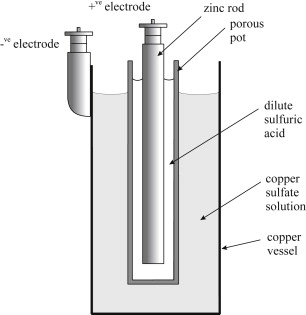
\includegraphics[width=0.7\linewidth]{Images/daniell}
            \caption{Daniell 전지}\label{f17}\cite{WINTERBONE2015497}
        \end{figure}
        \textbf{전해질 농도차 전지(Electrolyte concentration cell)}에서는 전해질의 농도를 제외하고 전극 칸의 구성이 동일하다. 한편 
        \textbf{전극 농도차 전지(Electrode concentration cell)}에서는 전극 그 자체가 서로 다른 농도를 가진다: 예를 들어, 서로 다른 압력으로 작동하는 
        기체 전극의 경우, 또는 아말감과 같이 동일한 물질로 이루어진 전극이지만 그 농도가 다른 경우이다. 
        \par Daniell 전지에서 두 전해질을 분리하는 다공성 용기와 같이, 서로 다른 두 전해질이 맞닿을 경우 생기는 전극 퍼텐셜을 \textbf{액간 전위(Liquid junction potential, $E_\mathrm{lj}$)}라 
        한다. 전해질 간 확산이 시작할 때, 두 이온의 이동도가 다르면 처음에는 더 큰 액간 전위가 형성된다. 
        이후 확산이 더 일어나면 특정 값으로 수렴하게 된다. 
        \par 염다리를 도입함으로써, 액간 전위를 1-2 mV 수준으로 줄일 수 있다. 염다리 내에 존재하는 이온의 
        이동도는 유사해야 한다. 이 경우 염다리 양쪽 끝의 액간 전위가 비슷해져, 서로 거의 상쇄된다.
        \par 전지는 다음과 같이 나타낸다:
        \begin{defn}[전지를 나타낼 때 쓰는 기호]
        \begin{enum}
            \item $\vert$ 상 또는 화학종 간 계면
            \item $\vdots$ 액간 계면
            \item $\vert \vert$ 액간 전위가 없다고 가정하는 계면
        \end{enum}
        \end{defn}
        따라서 Figure \ref{f17}의 전지는 다음과 같이 나타낼 수 있다:
        \begin{center}
            Zn(s) $\vert$ H$_2$SO$_4$(aq) $\vdots$ CuSO$_4$(aq) $\vert$ Cu(s)
        \end{center}
        \par 갈바니 전지에서는 자발적 화학 반응이 일어난다. 이때 \textbf{전지 반응(Cell reaction}은 
        오른쪽 전극이 환원 전극, 왼쪽 전극이 산화 전극일 때의 화학 반응이다. 이를 화학 반응식으로 나타내기 위해서는 오른쪽 전극의 반쪽 반응과 왼쪽 전극의 반쪽 반응을 환원 반응으로 나타낸 후에 왼쪽 전극의 반쪽 반응을 
        오른쪽 전극의 반쪽 반응에서 빼면 된다. 만약 전하 균형이 맞지 않을 경우 계수를 조정할 수 있다.
        \par 화학 평형에 도달하지 않은 전지 반응이 일어나는 전지에서는 외부 회로로 전자를 흘려보냄으로써 
        전기적 일을 할 수 있다. 주어진 양의 전자가 할 수 있는 일의 양은 전위차에 비례한다. 전체 반응이 평형에 
        도달하여 전위차가 발생하지 않은 전지는 할 수 있는 전기적 일이 없다.
        \par \ref{ch3sub4}에서 보인 것과 같이, $w_\mathrm{add,max} = \Delta G$에 해당한다. 전기화학에서는 추가적인 비팽창 일을 전기적 일($w_e$)로. 다루는 계는 전지로, 반응 Gibbs 에너지는 전지 반응의 Gibbs 에너지로 본다. 최대 일을 얻기 위해서는 반응이 가역적으로 일어나야 하므로, 여기에서는 
        반응이 가역적으로 일어난다고 본다. 또한 $\Delta_r G$는 $RT \ln Q$와 관련이 있으므로, 전지는 일정한 구성을 가지고 있다고 본다. 따라서 $\Delta_r G$를 구하기 위해서는 전지가 가역적으로, 일정한 구성으로 작동한다는 것을 가정해야 한다. 
        이때 전류는 흐르지 않는다. 이러한 가정을 통해 정의되는 전위차를 \textbf{전지 전위(Cell potential, $E_\mathrm{cell}$)}라 
        한다.
        \par 전지 전위는 다음과 같이 정의된다: 전지 반응이 $\difform \xi$만큼 일어났을 때, 식 \ref{rxngibbs}에 의해 
        \begin{equation*}
            \difform G = \Delta_r G \difform \xi
        \end{equation*}
        가 성립한다. 이때 $\difform G$는 최대 비팽창 미소 일에 해당하고, 이때 비팽창 일은 전기적 
        일에 해당한다:
        \begin{equation*}
            \difform w_e = \Delta_r G \difform \xi
        \end{equation*}
        이때 반응 1 mol 당 전자가 $\nu$ mol만큼 이동한다고 가정하자. $\difform \xi$만큼의 반응이 일어날 때 이동하는 전하량은 전자의 기본 전하량 $e$에 대해 $-\nu e N_\mathrm{A} \difform \xi$이다. 
        따라서 전기적 일 $\difform w = \phi \difform Q$에 대해, $\phi$는 전기 퍼텐셜에 해당하므로 $\phi = E_\mathrm{cell}$이다. 
        따라서 \textbf{Faraday 상수(Faraday's constant)} $F = e N_\mathrm{A}$로 정의하면, 
        다음이 성립한다:
        \begin{equation*}
            \difform w_e = -\nu F E_\mathrm{cell} \difform \xi
        \end{equation*}
        따라서 두 식에 의해, 다음이 성립한다:
        \begin{law}[전지 전위와 반응 Gibbs 에너지 사이의 관계]
        \begin{equation*}
            -\nu F E_\mathrm{cell} = \Delta_r G
        \end{equation*}
        \end{law}
        만약 전지 반응이 자발적이면(즉 $\Delta_r G < 0$이면), 전지 전위는 양수이다. 반대로, 만약 전지 반응의 반대 반응이 자발적이면(즉 $\Delta_r G > 0$이면), 전지 전위는 음수이다. 반응이 평형에 가까우면, 
        전지 전위는 매우 작다.
        \par 반응 Gibbs 에너지를 표준 반응 Gibbs 에너지와 비교한 식 $\Delta_r G = \Delta_r G^\circlehbar + RT\ln{Q}$에서, 양변을 $-\nu F$로 나누면 $E_\mathrm{cell} = \Delta_r G / \left(-\nu F\right)$에서
        \begin{equation*}
            E_\mathrm{cell}=-\frac{\Delta_r G^\circlehbar}{\nu F}-\frac{RT}{\nu f}\ln{Q}
        \end{equation*}
        이다. 이때 \textbf{표준 전지 전위(Standard cell potential, $E_\mathrm{cell}^\circlehbar$)}를 
        다음과 같이 정의한다:
        \begin{defn}[표준 전지 전위]
        \begin{equation*}
            E_\mathrm{cell}^\circlehbar = -\frac{\Delta_r G^\circlehbar}{\nu F}
        \end{equation*}
        \end{defn}
        따라서 다음이 성립한다:
        \begin{law}[Nernst 등식]
        \begin{equation*}
            E_\mathrm{cell} = E_\mathrm{cell}^\circlehbar - \frac{RT}{\nu F}\ln{Q}
        \end{equation*}
        \end{law}
        이 등식을 \textbf{Nernst 등식(Nernst equation)}이라 한다.
        \par $Q=K$일 때, $E_\mathrm{cell}=0$을 만족한다. 따라서 다음이 성립한다:
        \begin{law}[표준 전지 전위와 평형 상수 사이의 관계]
        \begin{equation*}
            E_\mathrm{cell}^\circlehbar = \frac{RT}{\nu F}\ln{K}
        \end{equation*}
        \end{law}
        이온의 표준 생성 Gibbs 에너지는 $\Delta_f G^\circlehbar\left(\text{H}^+\text{,aq}\right)=0$으로 정의한다. 이를 기준으로 반쪽 반응의 표준 환원 전위를 측정한다.
        \par 표준 전지 전위를 온도로 미분한 값은. $\displaystyle\left(\frac{\partial G}{\partial T}\right)_p = -S$에서 다음과 같이 유도된다:
        \begin{equation*}
            \frac{\difform E_\mathrm{cell}^\circlehbar}{\difform T}=\frac{\Delta_r S^\circlehbar}{\nu F}
        \end{equation*}
        이때 편미분이 아닌 이유는, 전지 반응은 압력에 무관하기 때문이다. 한편, 전지 반응의 반응 엔탈피를 구하는 방법은 다음과 같다:
        \begin{obs}[전지 반응의 반응 엔탈피]
        \begin{equation*}
            \begin{aligned}
                \Delta_r H^\circlehbar &=\Delta_r G^\circlehbar + T \Delta_r S^\circlehbar\\
                &= -\nu F\left(E_\mathrm{cell}^\circlehbar-T\frac{\difform E_\mathrm{cell}^\circlehbar}{\difform T}\right)
            \end{aligned}
        \end{equation*}
        \end{obs}
        따라서 전기화학적인 방법으로 전지 반응의 반응 엔탈피를 구할 수 있다.
        \section{전극 전위}
        \hspace{\parindent} 다음 전극을 \textbf{표준 수소 전극(Standard hydrogen electrode, SHE)}이라 하고, 이 전극의 표준 전극 전위를 모든 온도에서 $E^\circlehbar=0$으로 정의한다:
        \begin{defn}[표준 수소 전극]
        \begin{center}
            Pt(s) $\vert$ H$_2$(g) $\vert$ H$^+$(aq)
        \end{center}
        \end{defn}
        이때 수소 기체의 퓨가시티 $f_{\mathrm{H}_2} = 1$, 수소 이온의 활동도 $a_{\mathrm{H}^{+}}=1$이어야 한다. 
        산화-환원 쌍 X의 \textbf{표준 전위(Standard potential, $E^\circlehbar\left(X\right)$)}은 
        표준 수소 전극을 산화극으로 하는 다음과 같은 화학 전지의 표준 전지 전위로 정의한다:
        \begin{defn}[표준 전위]
        \begin{center}
            Pt(s) | H$_2$(g) | H$^{+}$(aq) || X, $E^\circlehbar\left(X\right)=E^\circlehbar_\mathrm{cell}$
        \end{center}
        \end{defn}
        표준 전지 전위는 두 전극의 표준 전위 차로 계산할 수 있다:
        \begin{obs}[표준 전지 전위]
        \begin{center}
            L $\vert \vert$ R, $E^\circlehbar_\mathrm{cell}=E^\circlehbar\left(R\right) - E^\circlehbar\left(L\right)$
        \end{center}
        \end{obs}
        \par 표준 전위를 구하는 방법을 Ag/AgCl 전극을 통해 알아보자. 다음과 같은 전지를 통해 측정한다:
        \begin{center}
            Pt(s) | H$_2$(g) | HCl (aq, $b$) | AgCl(s) | Ag(s)
        \end{center}
        이때 전체 반응은 다음과 같이 진행된다:
        \begin{center}
            $\displaystyle\frac{1}{2}$ H$_2$(g) + AgCl(s) $\rightarrow$ HCl(aq) + Ag(s)
        \end{center}
        따라서 표준 전지 전위는 다음과 같다:
        \begin{equation*}
            E^\circlehbar_\mathrm{cell}=E^\circlehbar\left(\text{AgCl/Ag,Cl}^{-}\right)-E^\circlehbar\left(\text{SHE}\right)=E^\circlehbar\left(\text{AgCl/Ag,Cl}^{-}\right),\, \nu=1
        \end{equation*}
        따라서 Nernst 등식은 다음과 같이 쓸 수 있다:
        \begin{equation*}
            E_\mathrm{cell}=E^\circlehbar\left(\text{AgCl/Ag,Cl}^{-}\right)-\frac{RT}{F}\ln{\frac{a_{\mathrm{H^+}}a_{\mathrm{Cl^-}}}{a_\mathrm{H_2}^{1/2}}}
        \end{equation*}
        만약 표준 상태라면, $a_\mathrm{H_2}=1$를 만족한다. 또한, $a_\mathrm{H^+}=\gamma_\pm b/b^\circlehbar$이고 
        $a_\mathrm{Cl^-}=\gamma_\pm b/b^\circlehbar$이므로 다음과 같이 쓸 수 있다:
        \begin{equation*}
            E_\mathrm{cell}=E^\circlehbar-\frac{RT}{F}\ln{\frac{{\gamma_\pm}^2 b^2}{{b^\circlehbar}^2}}
        \end{equation*}
        \begin{obs}\label{eqn268}
        \begin{equation*}
            E_\text{cell}+\frac{2RT}{F}\ln{\frac{b}{b^\circlehbar}}=E^\circlehbar-\frac{2RT}{F}\ln{\gamma_\pm}
        \end{equation*}
        \end{obs}
        이때, Debye-Hückel 한계 법칙에 의해 $b\rightarrow 0$일 때
        \begin{equation*}
            \log{\gamma_\pm}=-A\left\vert z_+ z_-\right\vert I^{1/2}=-A\left(b/b^\circlehbar\right)^{1/2}
        \end{equation*}
        가 성립하고, 따라서 식 \ref{eqn268}를 다시 정리하면
        \begin{equation*}
            E_\text{cell}+\frac{2RT}{F}\ln{\frac{b}{b^\circlehbar}}=E^\circlehbar\frac{2ART\ln{10}}{F}\left(\frac{b}{b^\circlehbar}\right)^{1/2}
        \end{equation*}
        이다. 이때 $\displaystyle C=\frac{2ART\ln{10}}{F}$로 두면 다음이 성립한다:
        \begin{equation*}
            E_\text{cell}+\frac{2RT}{F}\ln{\frac{b}{b^\circlehbar}}=E^\circlehbar + C\times\left(\frac{b}{b^\circlehbar}\right)^{1/2}
        \end{equation*}
        따라서 $\left(b/b^\circlehbar\right)^{1/2}$를 $x$축으로 하고 $E_\text{cell}+\frac{2RT}{F}\ln{\left(b/b^\circlehbar\right)}$을 $y$축으로 하여 선형회귀하면 $y$절편이 표준 전위에 해당하게 된다.
        \par 관여하는 전자 수가 다른 두 반쪽 반응을 결합하기 위해서는 다음과 같은 식을 이용한다:
        \begin{equation*}
            \nu_c E^\circlehbar\left(c\right)=\nu_a E^\circlehbar\left(a\right) - \nu_b E^\circlehbar\left(b\right)
        \end{equation*}
        이때 $\nu_r$은 각각의 반쪽 반응에서 관여하는 전자의 수이다.
        \par 화학 전지 L $\vert\vert$ R (즉 Ox$_L$/Red$_L$ $\vert\vert$ Ox$_R$/Red$_R$)이 있을 때, 다음 반쪽 반응과 표준 전지 전위를 관례적으로 이용한다:
        \begin{center}
            Ox$_R$ + $\nu$e$^- \rightarrow$ Red$_R$, Ox$_L$ + $\nu$e$^- \rightarrow$ Red$_L$
        \end{center}
        \begin{equation*}
            E_\text{cell}^\circlehbar = E^\circlehbar\left(R\right)-E^\circlehbar\left(L\right)
        \end{equation*}
        이때 전체 반응은 다음을 관례적으로 이용한다:
        \begin{center}
            R $-$ L : Red$_L+$ Ox$_R \rightarrow$ Ox$_L+$ Red$_R$
        \end{center}
        만약 이 반응의 $K>1$이면 $E_\text{cell}^\circlehbar$이고, $E^\circlehbar\left(R\right)>E^\circlehbar\left(L\right)$이다. 이 경우 Red$_L$이 Ox$_R$을 환원시키는 경향이 더 크다. 즉, 
        \textbf{$E^\circlehbar\left(R\right)>E^\circlehbar\left(L\right)$일 때 환원시키는 (즉 자신이 산화되는) 경향은 Red$_L$이 Red$_R$보다 더 크다.}
        \textbf{전위 서열(Electrochemical series)}은 금속 원소가 산화되는 경향성을 표준 전위를 기준으로 
        늘어 놓은 열이다.\footnote[17]{우리가 "칼카나마알아철니..."로 외우는 그 목록이 맞다.} 표준 전위가 낮을수록 금속 원소가 산화되는 (즉 다른 화학종을 환원시키는) 경향이 강하므로, 목록의 아래에 있을수록 환원제로 작용하는 경향성이 강하다.
        \par 마지막으로, Nernst 식을 이용하여 활동도 계수 및 평형 상수를 결정할 수 있다.